\section{Real-World Experiments}
\label{sec:experiments}

We evaluate \MethodName{} on four real-world manipulation tasks that require dexterous control and sub-millimeter precision. A pretrained VLA provides a strong initialization for most parts of these tasks, but success and speed ultimately depend on refining the critical contact-rich phase that demands the most precision. Our experiments test whether our method can deliver such improvements under the practical constraints that motivate the method: limited robot interaction time, sparse human supervision, and lightweight online learning.


We structure the evaluation around the following questions:
\begin{enumerate}
    \item[\textbf{Q1.}] Can \MethodName{} improve manipulation performance over the base VLA model?
    \item[\textbf{Q2.}] How does \MethodName{} compare to alternative RL approaches on these tasks?
    \item[\textbf{Q3.}] How much does each component of the method---the RL token, chunked action prediction, policy regularization, and reference-action pass-through---contribute to the method's performance?
    \item[\textbf{Q4.}] Does \MethodName{} enable the policy to discover a better strategy and how does its strategy compare to the original demonstration data? 
\end{enumerate}
% ===========================================================
\subsection{Tasks and Setup}
\label{sec:tasks}


We evaluate our method on the following tasks (Fig.~\ref{fig:tasks}):

\begin{itemize}[leftmargin=*, itemsep=2pt]
    \item \textbf{Screw installation.} The robot must use an electric screwdriver to drive an M3 screw into a threaded receptacle. This requires sub-millimeter alignment between the screw head and screwdriver tip. The task is especially difficult because (1) the screw may not always sit perfectly upright, (2) when holding the screwdriver, any rotation of the end effector is amplified by the 10\,cm distance between the screwdriver tip and the grasp point, and (3) critical visual cues are visible primarily from the wide-angle wrist camera on the opposite arm, presenting a challenging perceptual problem.
    
    \item \textbf{Zip tie fastening.} The robot must thread a zip tie tail through its narrow locking slot. This task involves coordinated bimanual control of a deformable object with tight tolerances. Successful insertion requires inferring the position of the tip and slot solely from the wrist cameras and executing with millimeter precision.
    
    \item \textbf{Ethernet insertion.} The robot must insert an Ethernet connector into a recessed port. This requires accurate positional and angular alignment, followed by a firm and decisive insertion motion. Small orientation errors or hesitant contact typically cause the connector to catch on the housing rather than insert into the port, making success sensitive to both precision and contact dynamics.
    
    \item \textbf{Charger insertion.} The robot must align and insert a charger into a power strip. The task is difficult because the policy must achieve centimeter-level alignment while not always having clear observability of the prongs and socket. Small alignment errors often lead to repeated probing or failed insertion attempts.

\end{itemize}

Each task includes grasping, repositioning, and alignment, and spans 30--120\,s (at 50\,Hz roughly 1500--6000 control steps). For each task, we identify the \emph{critical phase}---the insertion, fastening, or rotation segment---where precision requirements are the highest and where the base VLA most frequently slows down or fails. These phases typically last 5--20\,s (250--1000 control steps). 

\textbf{Critical-phase evaluation.}\quad
Since our method is designed to improve exactly these critical phases, we first focus our evaluation on comparing methods and ablations only on the critical phase. In this setting, episodes begin after being reset to a partially completed task state right before the critical phase, using a slightly randomized set of initial configurations. For example, in zip tie fastening, the robot begins already holding the two ends of the zip tie before the insertion attempt begins. This setup isolates the precision-critical segment where RL is expected to matter most, and reduces confounding variance from earlier phases of the task, such as grasping and transport, which are already handled reasonably well by the base VLA. Each agent is evaluated over 50 episodes per task in this controlled setting.

\textbf{Full-task evaluation.}\quad
Controlled critical-phase evaluation is useful for isolating the bottleneck that our method is designed to improve, but it does not capture the full variability of long-horizon execution. We therefore additionally evaluate full-task performance in a more realistic setting, where the robot starts from its ``home position'', executes the earlier stages of the task with the base policy, and enters the critical phase under the state variation induced by that execution. This setting is substantially harder, since the RL-improved behavior must remain effective under the broader distribution of states produced by the preceding policy. For the full-task training, we start by having RL focus on the critical phase with small randomization, and then move on to the full-task setting.

\textbf{Experiment Details.}\quad
The RL policy inputs consist of the RL token (produced from two wrist camera images and one base-camera image), and additional proprioceptive state. Depending on the task, this auxiliary state may include joint position (screw), end-effector pose (zip tie, Ethernet and charger). We use $\pi_{0.6}$~\cite{pi06_model_card} as the base VLA policy. The robot runs at a control frequency of 50\,Hz. With a 14-dimensional per-timestep action space, this corresponds to a 140-dimensional chunked action for the RL actor. We provide more implementation details in App.~\ref{app:exp}. 

% ===========================================================
%\subsection{Data and Training}

%Online RL training runs for 1--2 hours of wall-clock robot time per task. The first 5 minutes consist of VLA warmup rollouts (with human success/failure labels) to seed the replay buffer. During early RL rollouts, the human supervisor terminates visibly risky motions and occasionally intervenes via teleoperation to demonstrate recovery behaviors. All interventions are stored in the replay buffer alongside autonomous transitions. We use the same reward structure (human binary label) for all tasks and all methods.

% ===========================================================
\subsection{Baselines and Ablations}
\label{sec:baselines}
% ===========================================================



\begin{figure*}
    \centering
    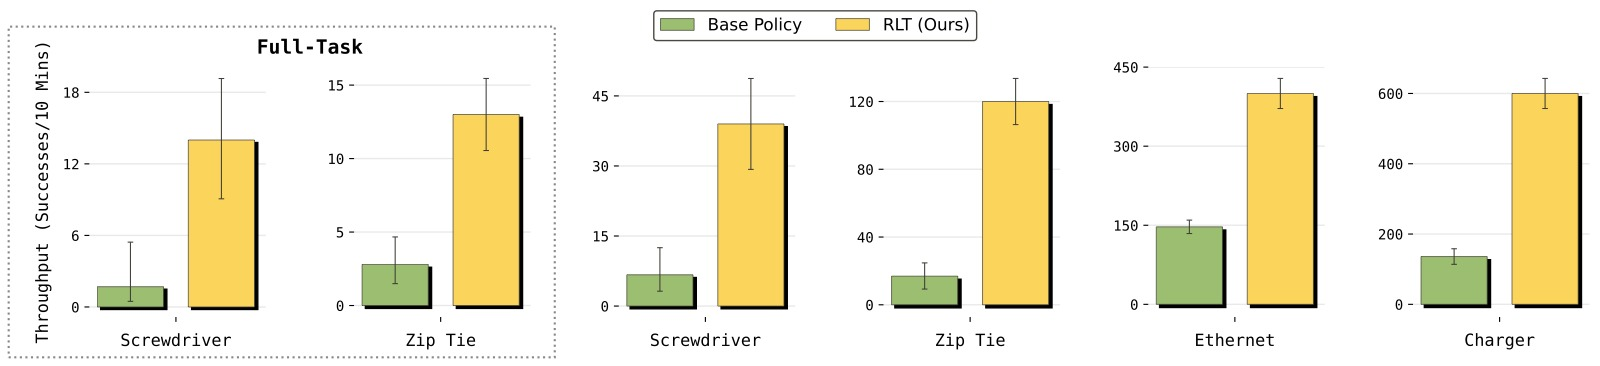
\includegraphics[width=1\linewidth]{figs/rlt_throughput_all.pdf}
    \caption{\textbf{\MethodName{} increases throughput significantly} over the base VLA policy, improving both the speed and consistency of the critical phase of each task. The improvement is especially pronounced for the harder tasks where the VLA policy is prone to making mistakes.}
    \label{fig:results_throughput}
\end{figure*}

\begin{figure*}
    \centering
    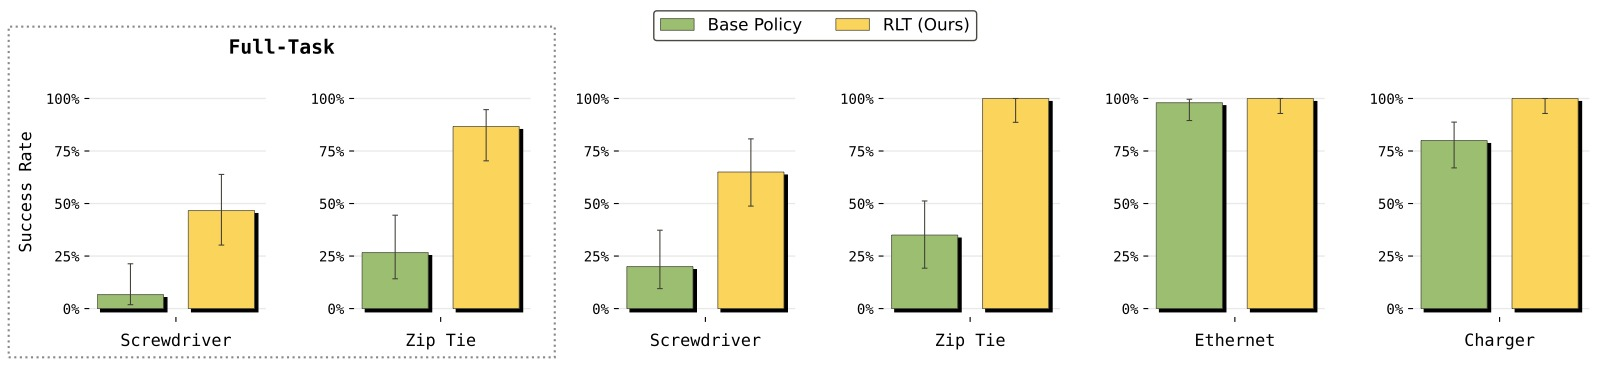
\includegraphics[width=1\linewidth]{figs/rlt_success_rate_all.pdf}
\caption{\textbf{\MethodName{} can boost success rates across multiple tasks}. Where the VLA is already competent (e.g., the Ethernet task) it maintains success rate and increases throughput. For tasks that are challenging for the base VLA policy (screwdriver and zip tie) \MethodName{} leads to a significant improvement in success.}
    \label{fig:results_success}
\end{figure*}

We start from a pretrained VLA model $\pi_{0.6}$~\cite{pi06_model_card}.
For each task, we collect $1$--$10$ hours of teleoperated demonstrations. We then fine-tune the VLA model while training our RL token representation.
%%SL.3.17: let's make sure we're using consistent terminology (do we call it feature head everywhere? if not, let's use the consistent term)
This produces the base VLA policy that we use throughout all of the experiments. We run RL training for between 400 and 1000 episodes depending on the task difficulty. Excluding reset and various overhead, each of the experiments produces approximately 15 minutes to 5 hours of actual robot data. We measure the performance in terms of the success rate on each task, judged by a binary reward signal from a human operator. We also report throughput, the number of successful task completions per 10 minute interval, in order to evaluate improvements in terms of both robustness and speed. We evaluate all tasks on their critical phases, and we evaluate the two harder tasks---the screw and zip tie tasks---in the full-task setting.

We compare \MethodName{} to four baseline methods that improve policies from experience. For fair comparisons, we train each RL method with the same amount of data (see App.~\ref{app:baseline}).

\begin{itemize}[leftmargin=*, itemsep=2pt]
    
    \item \textbf{HIL-SERL}~\cite{luo2024precise}: Like our method, HIL-SERL trains a small actor and critic with a combination of experience and interventions, but unlike \MethodName{}, it does not use representations from a pretrained VLA, instead using a simple ResNet encoder pretrained for standard computer vision tasks.
    \item \textbf{Probe-Learn-Distill}~\cite{xiao2025selfimprovingvisionlanguageactionmodelsdata}: PLD learns a residual policy that outputs a residual for each single-step action. It scales the residual by a hyperparameter and sums it with one step from the frozen VLA's action prediction to execute. 
    \item \textbf{DSRL}~\cite{Wagenmaker2025DSRL}: DSRL learns an online RL policy in the latent noise space of a flow VLA model. It ``steers'' the VLA action generation by selecting the noise to feed into the frozen VLA model's action generator. This method implicitly constrains exploration to those actions that can be generated by the VLA, and explores among its modes.
    \item \textbf{DAgger}~\cite{rossdagger,kelly2019hgdaggerinteractiveimitationlearning}: We fine-tune the base VLA model on the human intervention data collected during our training. 
    %%SL.3.17: doesn't that contradict the earlier statement that we use the same amount of data for all of them? (it's not necessarily a problem, just maybe change that sentence...)
    %%KK.3.17: updated
\end{itemize}
We also isolate the contribution of each component of our method by removing them individually:
\begin{itemize}[leftmargin=*, itemsep=2pt]
    \item \textbf{w/o RL token}: Replace the RL token with a frozen, ImageNet pretrained ResNet-10 encoder from \citep{luo2024serl}.
    \item \textbf{w/o Chunk}: The RL policy outputs single-step actions ($C{=}1$) instead of action chunks. Because this policy needs to run at 50\,Hz and querying the base VLA model at 50\,Hz would be infeasible, we have to replace the RL token with the ResNet-10 encoder. 
    \item \textbf{w/o BC Regularizer}: Set $\beta{=}0$ in Eq.~\eqref{eq:actor_loss}; the policy is trained with the $Q$-function alone.
    \item \textbf{w/o Pass-Through}: Remove $\tilde{\mathbf{a}}$ from the policy input in Eq.~\eqref{eq:policy}; the RL actor generates actions from state and RL token alone.
\end{itemize}

% ===========================================================
\subsection{Experimental Results}
\label{sec:results}


% ===========================================================


\begin{figure}
    \centering
    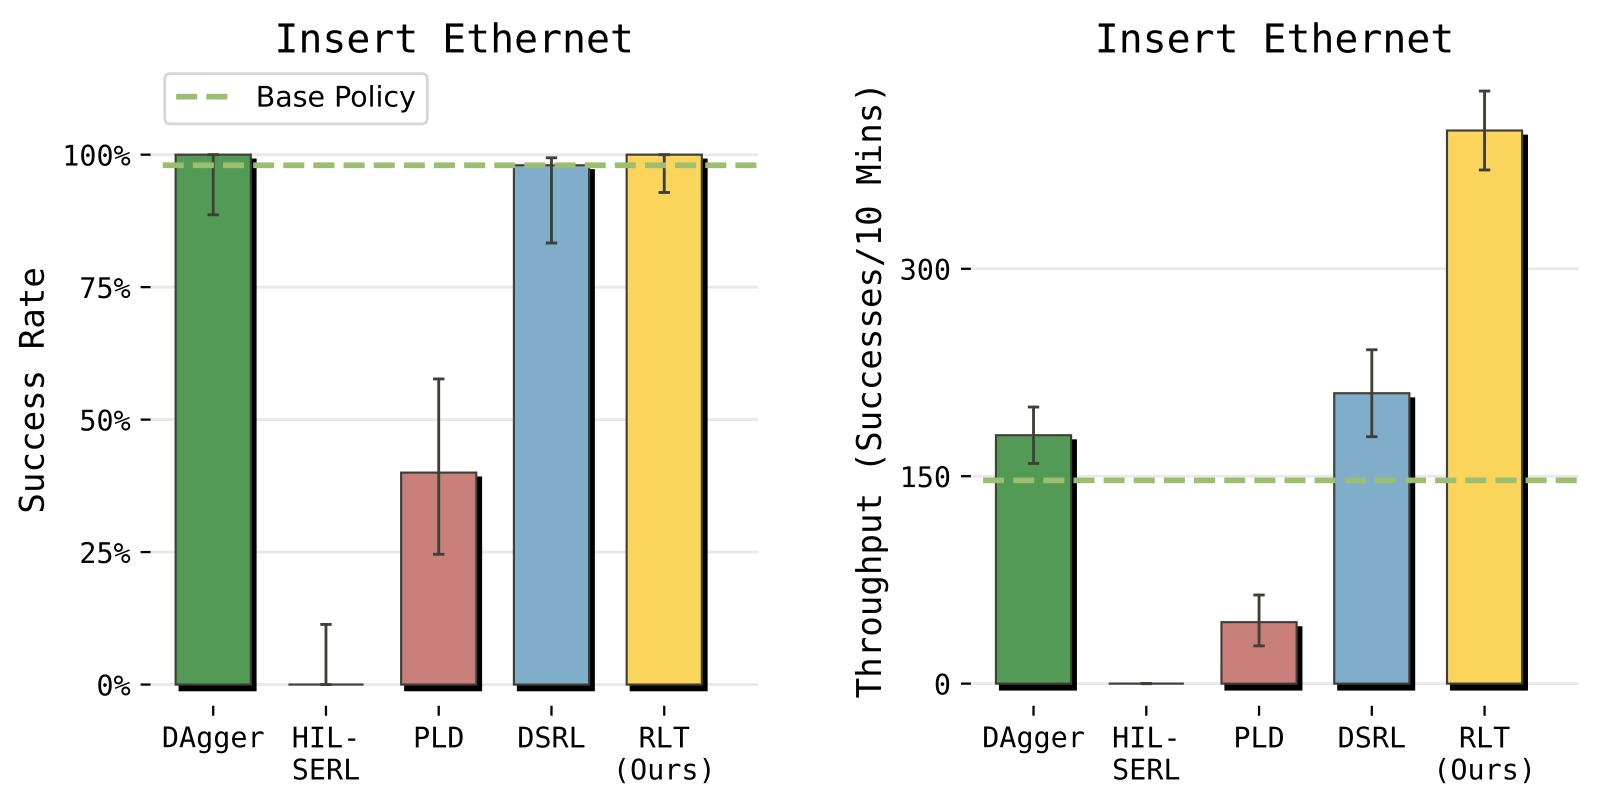
\includegraphics[width=\linewidth]{figs/method_comparison.pdf}
    \caption{\textbf{Comparison to other RL algorithms.} We compare \MethodName{} against several baselines from the recent RL literature. Methods that consider only single actions, rather than action chunks, (HIL-SERL, PLD) perform poorly. DSRL leads to high success but significantly lags behind in throughput.}
    \label{fig:baseline_comparison}
\end{figure}


% -----------------------------------------------------------
\textbf{Q1: Does online RL improve over the base VLA policy?}
% -----------------------------------------------------------
% ME: Maybe we should state more clearly that RLRT doesn't really improve the base policy outside the critical phase but it doesn't hurt performance so any improvement in the critical phase is a win overall. 
We evaluate our method in two regimes: the \emph{controlled} setting that isolates the critical phase and the \emph{full-task} setting that requires the RL policy to be more robust.
%%SL.3.17: I think we already explained this at the beginning of the experiments section, perhaps we could associate some term with it (controlled/full-task), and just refer to it here to avoid repetition?
\emph{Online RL improves success rate and execution speed of the base model} in both settings. In the controlled setting, \MethodName{} consistently improves the critical phase of all four tasks. Even on the relatively easier charger and Ethernet tasks, where the base policy already achieves good reliability, the policy learned by \MethodName{} is about $3{\times}$ faster in the critical phase. The boost to success rate is more pronounced on the harder zip tie and screwdriver tasks.  In the full-task evaluation, overall success rates are lower due to compounding errors from earlier parts of the task (grasping/lifting objects etc.), but \MethodName{} still improves the success rate by 40\% on the screwdriver task and 60\% on the zip tie task.

% \begin{table}[t]
% \centering
% \label{tab:main}
% \resizebox{0.8\linewidth}{!}{
% \begin{tabular}{l cc}
% \toprule
% % & \multicolumn{2}{c}{\textbf{Ethernet}} \\
% % \cmidrule(lr){2-3}
% Method & Success Rate (50 trials) & Steps \\
% \midrule
% Base SFT Policy     & 98\% & 200 \\
% \midrule
% DAgger              & \textbf{100\%} & 167 \\
% HIL-SERL~\cite{hil-serl}            & 0\% & -- \\
% PLD~\cite{pld}                 & 40\% & 270 \\
% DSRL~\cite{dsrl}                & 98\% & 140 \\
% \MethodName{} (Ours)       & \textbf{100\%} & \textbf{70} \\
% \bottomrule
% \end{tabular}
% }
% \caption{\textbf{Controlled-phase evaluation.} Success rate (\%) and mean steps to completion ($\downarrow$) over 50 episodes.}
% \end{table}
% ---------------------------------------------
\textbf{Q2: How does \MethodName{} compare to alternative methods?}
% -----------------------------------------------------------
As shown in Fig.~\ref{fig:baseline_comparison}, \emph{\MethodName{} results in a significant boost to throughput compared to baselines}. We compare against four baselines on the Ethernet task. HIL-SERL and PLD---both single-step online RL methods---fail to learn effectively on this task, which spans hundreds of steps with a sparse reward. Without action chunking, the horizon of the task is very long, and the value function updates are ineffective at propagating the sparse reward signal. For this simpler task, DAgger and DSRL achieve success rates comparable to \MethodName{} (Fig.~\ref{fig:baseline_comparison}), but provide significantly less improvement in terms of speed. DAgger is an imitation learning method, and is limited to the speed of the human demonstrations and interventions. DSRL is an RL method that strongly constrains the policy to remain close to the base VLA, providing stable training but comparatively less potential for improvement.  In contrast, \MethodName{} matches the base policy's high success rate while reducing mean steps to completion by $2{\times}$ over the base policy.

%improves consistency where the base policy's failures are occasional misalignments, but cannot discover faster strategies since it is bounded by human demonstration speed, and provides limited gains on tasks requiring fundamentally new behaviors (e.g., precise rotation). HIL-SERL shares our human-in-the-loop RL framework but operates at the single-step level; on tasks spanning hundreds of steps with sparse reward, its critic fails to propagate useful gradients within the available interaction budget. Residual RL is competitive when its hand-tuned residual scales happen to match the required correction magnitude, but the same scales that work for one task can be too conservative or too aggressive for another---precisely the task-specific scaffolding \MethodName{} eliminates. Latent Noise RL improves execution consistency by modulating diffusion noise, but cannot discover strategies outside the VLA's pretrained distribution, such as the faster insertion motions \MethodName{} learns.


%\textbf{DAgger} improves reliability on tasks where the base policy's failure mode is inconsistency (e.g., occasionally misaligning), but it cannot discover faster strategies since it is bounded by the speed of human demonstration. On Screw Installation and Zip Tie Fastening, where the VLA's failure mode is more fundamental (inability to execute precise rotation consistently), DAgger provides limited gains.

%\textbf{HIL-SERL}, despite sharing the human-in-the-loop RL framework, struggles with the long effective horizon: operating at the single-step level on tasks spanning hundreds of steps with sparse binary reward, the critic fails to propagate meaningful gradients within the available interaction budget. It achieves improvements on [shorter/simpler task] but shows limited progress on longer-horizon tasks.

%\textbf{Residual RL} is competitive on [task], where its hand-tuned residual scales happen to match the required correction magnitude. However, the same scales that work for one task can be too conservative for another (preventing sufficient exploration) or too aggressive (causing instability). This task-specificity is precisely the scaffolding \MethodName{} aims to eliminate.

%\textbf{Latent Noise RL} effectively optimizes within the VLA's existing behavioral modes and can improve execution consistency. However, because it only modulates the diffusion noise, it cannot discover strategies outside the VLA's pretrained distribution---such as the faster, more decisive insertion motions that \MethodName{} learns.

% -----------------------------------------------------------
\textbf{Q3: How much does each component contribute?}
% -----------------------------------------------------------
% ME: I dont know if it is very clear that no RL head = resnet 10 encoder. Maybe we should change the text or plot to match. Also the no rl head + no chunking results are confounded which makes the claims around chunk size somewhat questionable.
\emph{All four design choices---RL token, action chunks, the BC regularizer, and reference-action pass-through---contribute meaningfully}.
%%SL.3.17: can we be more careful with jargon and phrasing? let's try to use self-explanatory terms, and use *consistent* terms throughout the paper (e.g., do we call it BC constraint before? do we call it reference pass-through? reference pass-through of what?)
%% Tobi: let's not call it constraint since it really isn't, I think we wrote regularizer above?
We validate that each component of our recipe provides a positive contribution (Fig.~\ref{fig:ablation_throughput}): replacing the RL token with a ResNet-10 encoder reduces throughput by $50$\%, confirming that our token encodes manipulation-relevant structure that an off-the-shelf encoder trained on standard computer vision tasks does not provide. Replacing chunks ($C{=}10$) with single-step actions dramatically increases the effective horizon of the task, since the value function needs to perform credit assignment over a much longer horizon. It also would make it infeasible to run our method with the RL token. In practice, the single-step variant cannot reliably match the base policy performance. %This is consistent with prior findings that sparse-reward RL at 50\,Hz requires far more data~\cite{li2025chunkrl}. 
Removing the BC regularizer ($\beta{=}0$) causes the largest single drop in performance, since it forces the actor to explore the full action space with only gradients from the $Q$-function. Removing the reference-action pass-through slows down learning, leads to early exploration drift, and occasionally degenerate behaviors. This ablation does eventually match the performance of \MethodName{} for this simpler task, but experiences more failures during the training process, as seen on the learning curve in Fig.~\ref{fig:ablation_throughput}.
%%SL.3.17: this is reasonable, but do we have quantitative results of this? learning curves or something?
%%KK.3.17: see Lcurve.


% \begin{table}[t]
% \centering
% \label{tab:ablation}
% \resizebox{0.9\linewidth}{!}{
% \begin{tabular}{l cc}
% \toprule
% Variant & Success Rate (50 trials) & Steps \\
% \midrule
% \MethodName{} (ours)       & \textbf{100\%} & \textbf{70} \\
% w/o RL Feature Head        & \textbf{100\%} & 250 \\
% w/o Reference Pass-Through & \textbf{100\%} & \textbf{70} \\
% w/o KL Constraint          & 0\% & -- \\
% w/o RL Head \& w/o Chunk   & 88\% & 205 \\
% \bottomrule
% \end{tabular}
% }
% \caption{\textbf{Ablation study (Ethernet).} Success rate (\%) and mean steps to completion ($\downarrow$) over 20 episodes. Best results in \textbf{bold}.}
% \end{table}


% \begin{figure}[t]
%     \centering
%     \begin{subfigure}[t]{0.48\linewidth}
%         \centering
%         \includegraphics[width=\linewidth]{figs/abalation_SR.png}
%         \caption{Success rate (\%)}
%         \label{fig:ablation_sr}
%     \end{subfigure}
%     \hfill
%     \begin{subfigure}[t]{0.48\linewidth}
%         \centering
%         \includegraphics[width=\linewidth]{figs/abalation_speed.png}
%         \caption{Mean steps to completion ($\downarrow$)}
%         \label{fig:ablation_speed}
%     \end{subfigure}
%     \caption{\textbf{Ablation results on Ethernet.} Performance comparison across model variants.}
%     \label{fig:ablation_combined}
% \end{figure}
\begin{figure}
    \centering
    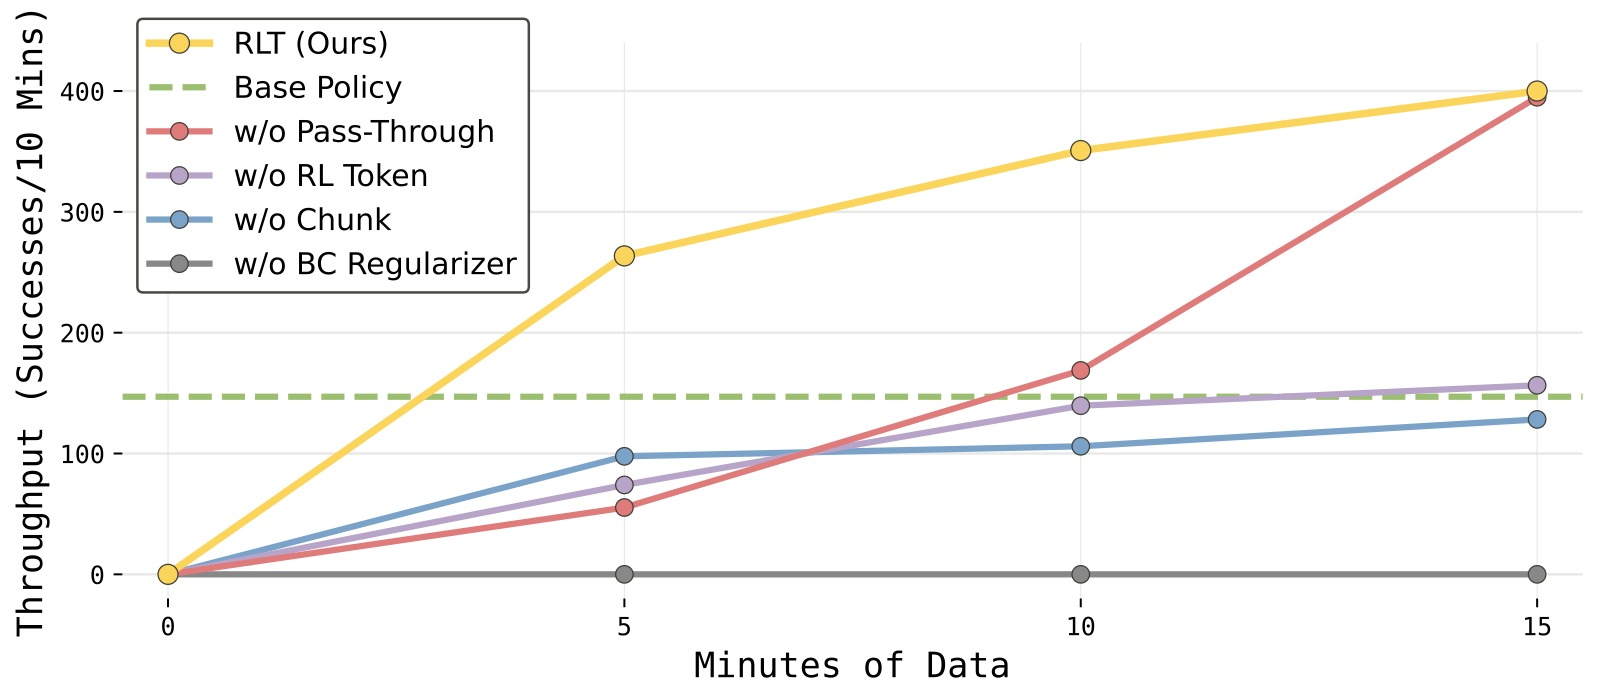
\includegraphics[width=1\linewidth]{figs/throughput_ablations.pdf}
    \caption{\textbf{Throughput at different points in training for Ethernet task.} The ablation study shows that each part of our method is important for good performance, and the full system learns fastest and performs best at the end. Notably, \MethodName{} outperforms the alternative policy after consuming only 5 minutes of data on the critical part of the task (total experiment time $\sim$ 40mins). Dropping the reference action from the actor input (``w/o Pass-Through'') still allows reaching the best final performance, but at the cost of slower learning and significantly more failures over the course of training. }
    \label{fig:ablation_throughput}
\end{figure}
\begin{figure}
    \centering
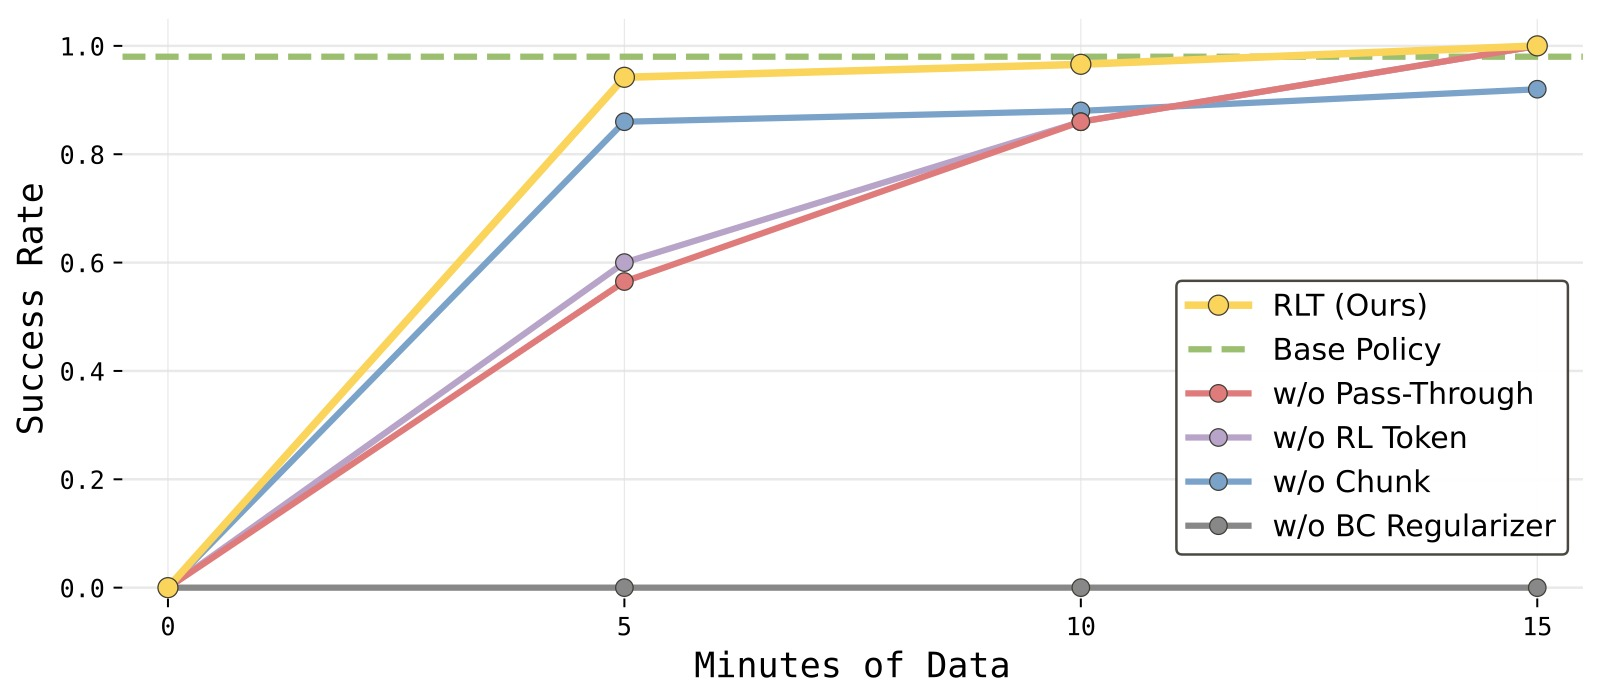
\includegraphics[width=1\linewidth]{figs/success_rate_ablations.pdf}
    \caption{\textbf{Success rate evaluation during training for the Ethernet task.} \MethodName{} quickly matches the success rate of the VLA policy on the Ethernet insertion task, while boosting throughput. Not using the reference-action pass-through or not using the RL token leads to slower learning.}
    \label{fig:placeholder}
\end{figure}

% -----------------------------------------------------------
\textbf{Q4: Does \MethodName{} lead to more effective emergent strategies?}
\begin{figure}
    \centering
    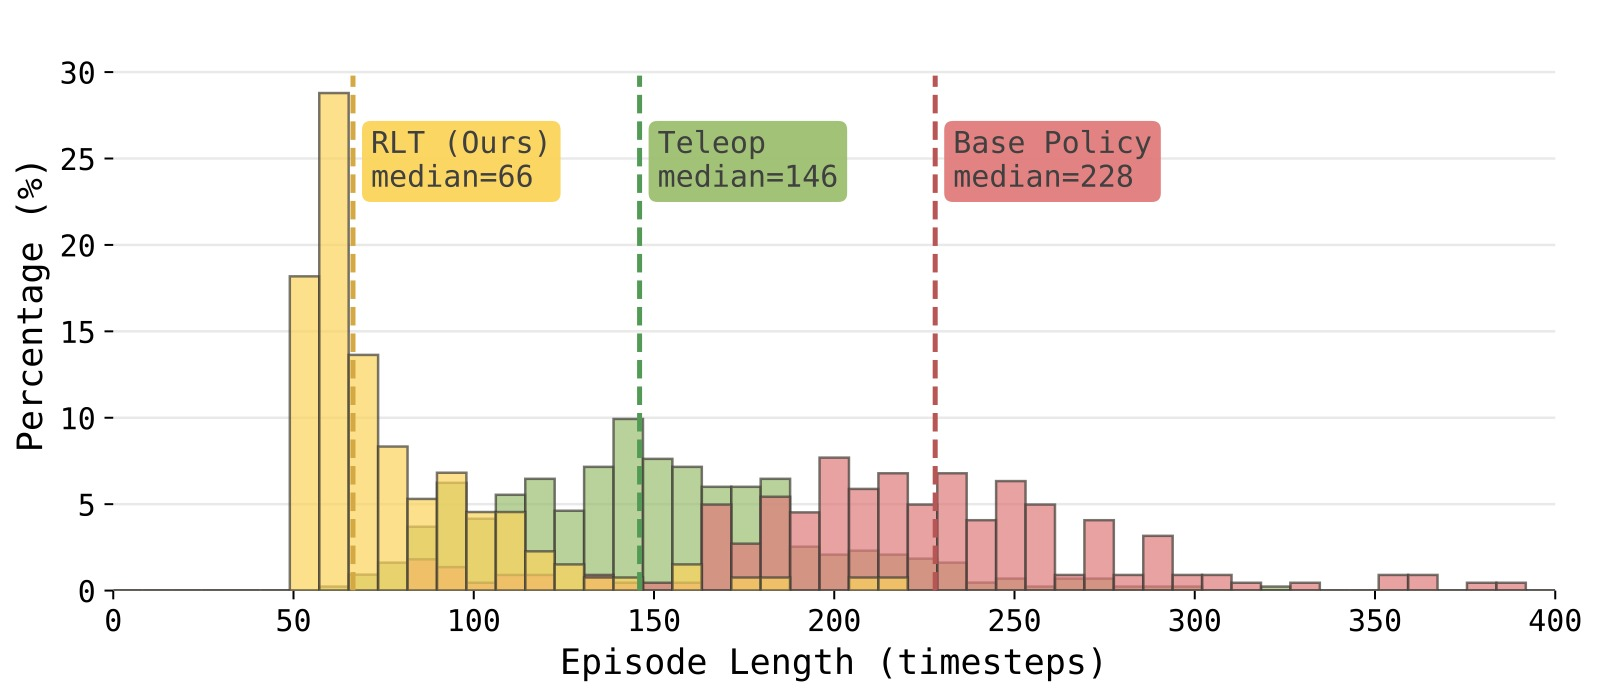
\includegraphics[width=1\linewidth]{figs/episode_length_histogram.pdf}
    \caption{\textbf{Speed on the Ethernet task.} \MethodName{} significantly improves the speed of the Ethernet task. The final policy is faster even than the demonstrations produced by expert teleoperators, and significantly faster than the base VLA model. Half of the RL episodes during the critical insertion phase (yellow) are faster than all of the teleoperated demonstrations (green).}
    \label{fig:speed}
\end{figure}
Beyond aggregate metrics, the  effect of online RL is a qualitative change in \emph{how} the robot performs the task. On the critical phase for the Ethernet task, we visualize the distribution of speeds for the teleoperated demonstrations, the base policy, and the final RL policy (Fig.~\ref{fig:speed}). The base VLA frequently exhibits ``probing'' behavior near contact: it approaches the target, retreats slightly, readjusts, and attempts again---sometimes cycling through several such attempts before succeeding. \MethodName{} instead approaches the port, and inserts the connector in a fluid motion. Even when it fails on the first attempt, \MethodName{} applies  pressure and wiggles the connector slightly to exploit compliance, leading to faster insertion. This behavior is not seen in the demonstration data and emerges purely from online exploration, illustrating that the method can go beyond imitating human strategies.


%\textbf{Emergent strategies.}\quad On [Task], we observe the RL policy discovering 
%\kk{How are we benefiting long-horizon task: (brainstorming) we key switch to apply the method to the critical stage, we show that we are better than the baseline SFT policy on the full task.  (note that with key switch we have much more randomization in the initial config because of compounding error in the imitation policy and the learning can be more challenging)}


\iffalse %%%%%
The controlled-phase experiments isolate the contact-critical segment to enable fair comparison; we now verify that gains compose into end-to-end improvements.

We select \textbf{[Task Name]} for the full-horizon evaluation, in which the robot must complete the entire manipulation pipeline---grasping, transport, alignment, and insertion---from a fully randomized initial configuration. Table~\ref{tab:distill} compares three policies:
\begin{itemize}[leftmargin=*, itemsep=2pt]
    \item \textbf{Base SFT}: The VLA fine-tuned on 5\,h of demonstration data.
    \item \textbf{RL Policy}: The RL policy head from \MethodName{}, operating on top of the frozen VLA during the contact phase only (the VLA handles earlier phases autonomously).
    \item \textbf{Distilled VLA}: The base VLA fine-tuned on the union of the original demonstrations and successful trajectories collected during online RL.
\end{itemize}

\begin{table}[t]
\centering
\caption{\textbf{Full-horizon evaluation on [Task Name].} Success rate (\%) and mean episode duration over 20 fully randomized episodes.}
\label{tab:distill}
\begin{tabular}{l c c}
\toprule
Policy & Success (\%) & Duration (s) \\
\midrule
Base SFT         & $p$ & -- \\
RL Policy        & $q$ & -- \\
Distilled VLA    & $\mathbf{r}$ & -- \\
\bottomrule
\end{tabular}
\end{table}

The RL Policy improves success rate from $p$\% to $q$\% on the full-horizon task, confirming that contact-phase improvements directly translate to end-to-end gains. The Distilled VLA---which absorbs the RL-collected data back into the foundation model via supervised fine-tuning---achieves $r$\% success, demonstrating the \emph{data flywheel} effect: online RL generates high-quality, in-distribution trajectories that improve the VLA itself, producing a single policy that handles the entire task without the RL head at inference time.

\fi


